\section{Class Exercises}
\subsection{Characteristics of a good Survey}
\begin{itemize}
    \item There is no up-to-date or survey paper published in the research domain
    \item There is a more compelling storyline and technical  direction
    \item One conducted in an interesting area of research with reasonable traction
    \item Judiciously pivots on the four cardinal objectives of storytelling
    \item A good survey will have sufficient models or methodologies to foster a comprehensive understanding of the subject research area.
\end{itemize}

\subsection{Story Writing with Closed Eyes}
Generalizability of 3D genomic structure techniques across species and the potential for a sustainable consensus.


\subsection{Redux - Using The Inner Child Language}
What happens if the 3D genomic structure techniques are not even generalizable across species?

\section{Examination of Domain Survey Papers}
\subsection{3C and 3C-based techniques: the powerful tools for spatial genome organization deciphering}
Han et al. \cite{han_3c_2018} heralded the first fully immersive survey in the foundational three-dimensional (3D) genomic architecture research domain. This survey discussed a comprehensive overview of the Chromosomes Conformation Capture (3C) and 3C-based techniques, which are essential tools for studying 3D genomic organization. Five techniques comprising 3C, 4C, 5C, ChIA-PET, and HiC were discussed as technologies that allow the capture of interactions between distal DNA regions, uncovering and emphasizing the influence of chromatin organization on genome stability and gene regulation. The authors provided sufficient analysis contrasting the different methods, highlighting their merits and demerits. They also made certain to guide the minds of their audience into an imaginative stance of the future of improving the quality of genome-wide chromatin interaction studies.
\subsubsection{The Story}
The paper tells the story of how advancing 3C-derived technologies have transformed the ability of researchers to explore the 3D organization of genomes, ultimately revealing hidden relationships between gene function and chromatin structure.

\subsection{Deciphering Hi-C: From 3D Genome to Function}
Being the frontier three-dimensional organization study technique at the time of this survey, Kong et al. \cite{kong_deciphering_2019} reviewed Hi-C technology and its ability to map genome-wide chromosomal interactions for an in-depth deciphering of 3D genomic architectures. The authors compared five major derivatives of the Hi-C technologies, emphasizing the specific adaptations for resolution enhancement, focus, or accuracy that each variant offers. The paper also discussed the improved analytic potential when Hi-C data is hybridized with other omics technologies, including cell fate determination, the relationship between biological functions and gene regulation, and disease mechanisms. Furthermore, the survey provided empirically proven recommendations regarding the best-fit methods for specific 3D genome studies.

\subsubsection{The Story}
The story advanced by the authors tells of the revolutionization of 3D genome exploration championed by the Hi-C technology, and how it bridges the gap between chromosomal architecture and gene function, while identifying limitations that must be addressed to comprehend genome dynamics fully.

\subsection{Computational Methods for Analyzing and Modeling Genome Structure and Organization}
In 2019, Lin et al. \cite{lin_computational_2019} conducted a survey in which various 3C-based developed computational methods for chromatin conformation data analysis was examined. The authors highlighted the advancements and challenges in detecting key features of the genome organization including topologically associating domains (TADs), loops, and A/B compartments, while stressing the role of computational models in capturing these interactions. Most importantly, this work reviewed the pros and cons of various approaches, spotlighting the significance of integrating multiple experimental data types to improve genome modeling accuracy as well as refine the understanding of dynamic chromatin behaviors. This survey, however, lacks a detailed comparative evaluation and essential details of technical nuances.
\subsubsection{The Story}
The paper's storyline is designed to tell how computational tools are evolving to decode 3D genomic structures, aiming to bridge the gap between experimental data and functional insights into chromosomal organization and, consequently, its biological relevance and implications.


\subsection{Deep Learning: New Computational Modelling Techniques for Genomics}
Eraslan et al. \cite{eraslan_deep_2019} explores the transformative impact of deep learning methods in genomics research, specifically improving tasks such as predicting the impact of genetic variation on gene regulation, DNA accessibility, and splicing. The paper dissects four major deep learning techniques including fully connected, convolutional, recurrent, and graph-convolutional neural networks while discussing their applications in integrating multiple data modalities, such as gene expression and chromatin accessibility. The paper then redressed major challenges in training deep learning models including data scarcity and computation complexities, highlighting how transfer learning and autoencoders can overcome these limitations.
\subsubsection{The Story}
This work pivots its story on how deep learning has revolutionized the field of genomics, advancing new tools to reveal complex patterns in genomic data, and enabling the prediction of molecular phenotypes and offering new possibilities for functional genomics research.

\subsection{An Overview of Methods for Reconstructing 3-D Chromosome and Genome Structures from Hi-C Data}
This author \cite{oluwadare_overview_2019} reviews various computational methods to infer three-dimensional genome structures from Hi-C data, categorizing them into distance-based, contact-based, and probabilistic models.
It highlights the progression from simple models like Multidimensional Scaling (MDS) to more advanced approaches that use optimization and probabilistic methods to predict genome architecture. The authors focused on methods that address key challenges, such as noise and resolution in Hi-C datasets. 
The authors discuss the need for further development in accuracy and scalability to handle large datasets and improve the biological relevance of predicted genome structures. This paper has received 132 citations, making it the most cited work in this collection. This is not surprising, as the survey extensively reviewed twenty computational models and is one of the most recent surveys in the 3D genome structure research domain. It was published in the BMC Bioinformatics journal, which has an h5-index of 76.
\subsubsection{The Story} This paper tells how computational methods have evolved to reconstruct 3D chromosome structures from Hi-C data, striving to overcome technical challenges and improve the resolution and biological accuracy of genome models.

\subsection{Predicting Genome Architecture: Challenges and Solutions}
In this survey, Belokoptova and Fishman \cite{belokopytova2021predicting} discussed using multiple computational methods, particularly polymer physics and machine learning models for predicting 3D genome architecture. They highlighted the limitations of existing models, ranging from insufficiency in the understanding of biophysical mechanisms to bottlenecks with generalizing models across cell types. This paper highlights computational challenges in simulating large-scale genome structures and the need to integrate high-resolution experimental data to improve prediction accuracy. Having been published in a highly reputable journal in 2021, this work has earned 38 citations. This survey is not as highly cited as Oluwadare et al. \cite{oluwadare_overview_2019} because its scope is not as broad. 
\subsubsection{The Story}
This paper tells the story of how computational methods have attempted to predict complex genomic structures and how they have continually improved to navigate challenges in modeling chromatin dynamics and explore new strategies to overcome the gaps in current scientific understanding. However, these gaps are still yet to be sufficiently addressed.
\begin{figure}[h!]
    \centering
    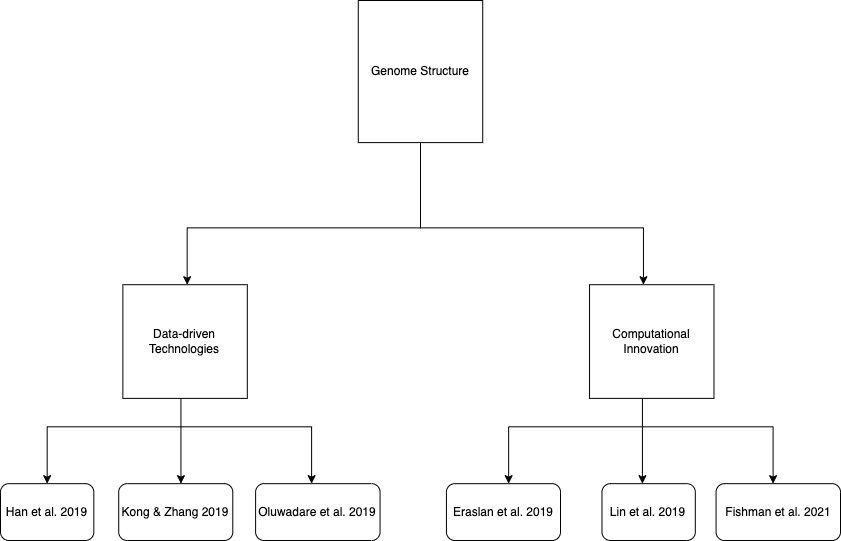
\includegraphics[width=1\textwidth]{images/j333.png}
    \caption{A tree representation of the broad categorization of review paper discussed.}
    \label{j3categories}
\end{figure}

\section{Potential Survey Paper Stories}
\begin{itemize}
    \item Chromatin Landscape exploration across species
    \item Cross-disciplinary survey on deep learning integration in terms of the generalizability of performing deep learning models for resolution enhancement in Hi-C to Micro-C
    \item Micro-C potential for exploring single-cell chromatin heterogeneity at nucleosome resolution and how that might differ from Hi-C in single-cell genomics.

\end{itemize}

\nocite{*}

